\subsection{Linear Simulation}
\label{subsec:lin_sim}
%\textcolor{red}{Yazdi's method and results}

In order to grasp the concept of the computer vision, a linear simulation program is developed in MATLAB. The simulation program is also used to preliminary test the chosen strategy before the code implementation into the paparazzi system. This simulation also gives our team possibility to easily test the strategy in various setups of the field at the tournament. 

\subsubsection{Model and Setup}
\textbf{The tournament field} is modeled based on our observation of the cyberzoo and the rules stated in the first announcement of the tournament. It is a 10 x 10 meter square field, with a smaller 7 x 7 meter square as the obstacle field , symmetrically placed inside, as shown in three example in Figure\ref{f:TopViewSamples}.

\textbf{Poles}, our initial assumption of the possible obstacle, are placed inside the obstacle field. Since there are no setup information, we choose to randomize the pole initial parameters, i.e., the pole number, the pole diameter and the x-y position, as shown in the table\ref{t:RandomPole} below. The ranges of position (x,y) are set to make the whole body of a pole to always be inside the obstacle area, considering the diameter ranges. Note that the origin of the field model is on the bottom-left. A limitation is added in the randomization process, so that each pole are always separated by at least a certain distance, which is assumed to be 2 times the diameter of the drone. This last assumption actually limit the number of pole that can be put inside the obstacle field: we found out that randomly positioning more than 10 poles is very difficult. The height of the pole is assumed  to be constant, i.e., 2 meters high. 

\begin{table}
\caption{Range of pole parameters randomization in the linear simulation}
\label{t:RandomPole}
\begin{center}
\begin{tabular}{lcc}
\hline \hline
Parameter & Range & Unit \\\hline
Pole number & 4 - 10 & - \\
Diameter & 40 - 60 & cm \\
Positions (x,y) & 2.1 - 7.9 $^*$ & m \\\hline\hline
\end{tabular}
\end{center}

\end{table}

\textbf{The Drone} is modeled from the observation of the AR-drone quad-rotor. Four circles with a heading indicator is used to visualized the drone with diameter of 0.4 m, in a top-down view as shown in Figure~\ref{f:TopViewSamples}. The drone motion is modeled using only linear kinematic equations with velocity changes, treating the drone as a point mass. Heading orientation is added to support the camera-view model, explained in the next paragraph. The model also consist of a random addition for the direction in each time step to simulate Drone drifting in the real life. 

It should be noted that the initial idea is to make a complete non-linear mathematical model of the drone using simulink, and hence to have a nonlinear simulation system. However, this is proven to be very difficult and time consuming, especially in determining the PID gain for its stability, and therefore was dropped. The focus of this simulation program then is only to test the strategy in various obstacle setups. The dynamic non-linear simulation will be conducted using paparazi simulator instead. 

\textbf{Camera-view} is modeled based on the pin-hole camera model, coupled with the specification of the AR-drone front camera. The result can be observed, from a random position of obstacle, in Figure~\ref{f:CameraViewSamples}. Further calibration is conducted to match the result with the sample pictures (Figure~\ref{f:Calibrations}) taken from zero altitude with a pole positioned 0.5, 1 and 2 meters infront of the camera. The calibrations results in a field of view (rounded) of 44 degree vertically, and 77 degree horizontally, as also shown by the dashed line coming from the front of the drone, in the top-down view Figure~\ref{f:TopViewSamples}. The poles are modeled as straight rectangles with specific width dictated by the randomization of poles, with a constant 2 meters of height. The color of the pole is not considered in the simulation, assuming a perfect detection of pole width. The floor is illustrated using straight lines, from the camera bottom field until the horizon at the bottom edge of the tournament field. The lines are always in the direction of the drone and only served as an illustration.

\begin{figure}[h]
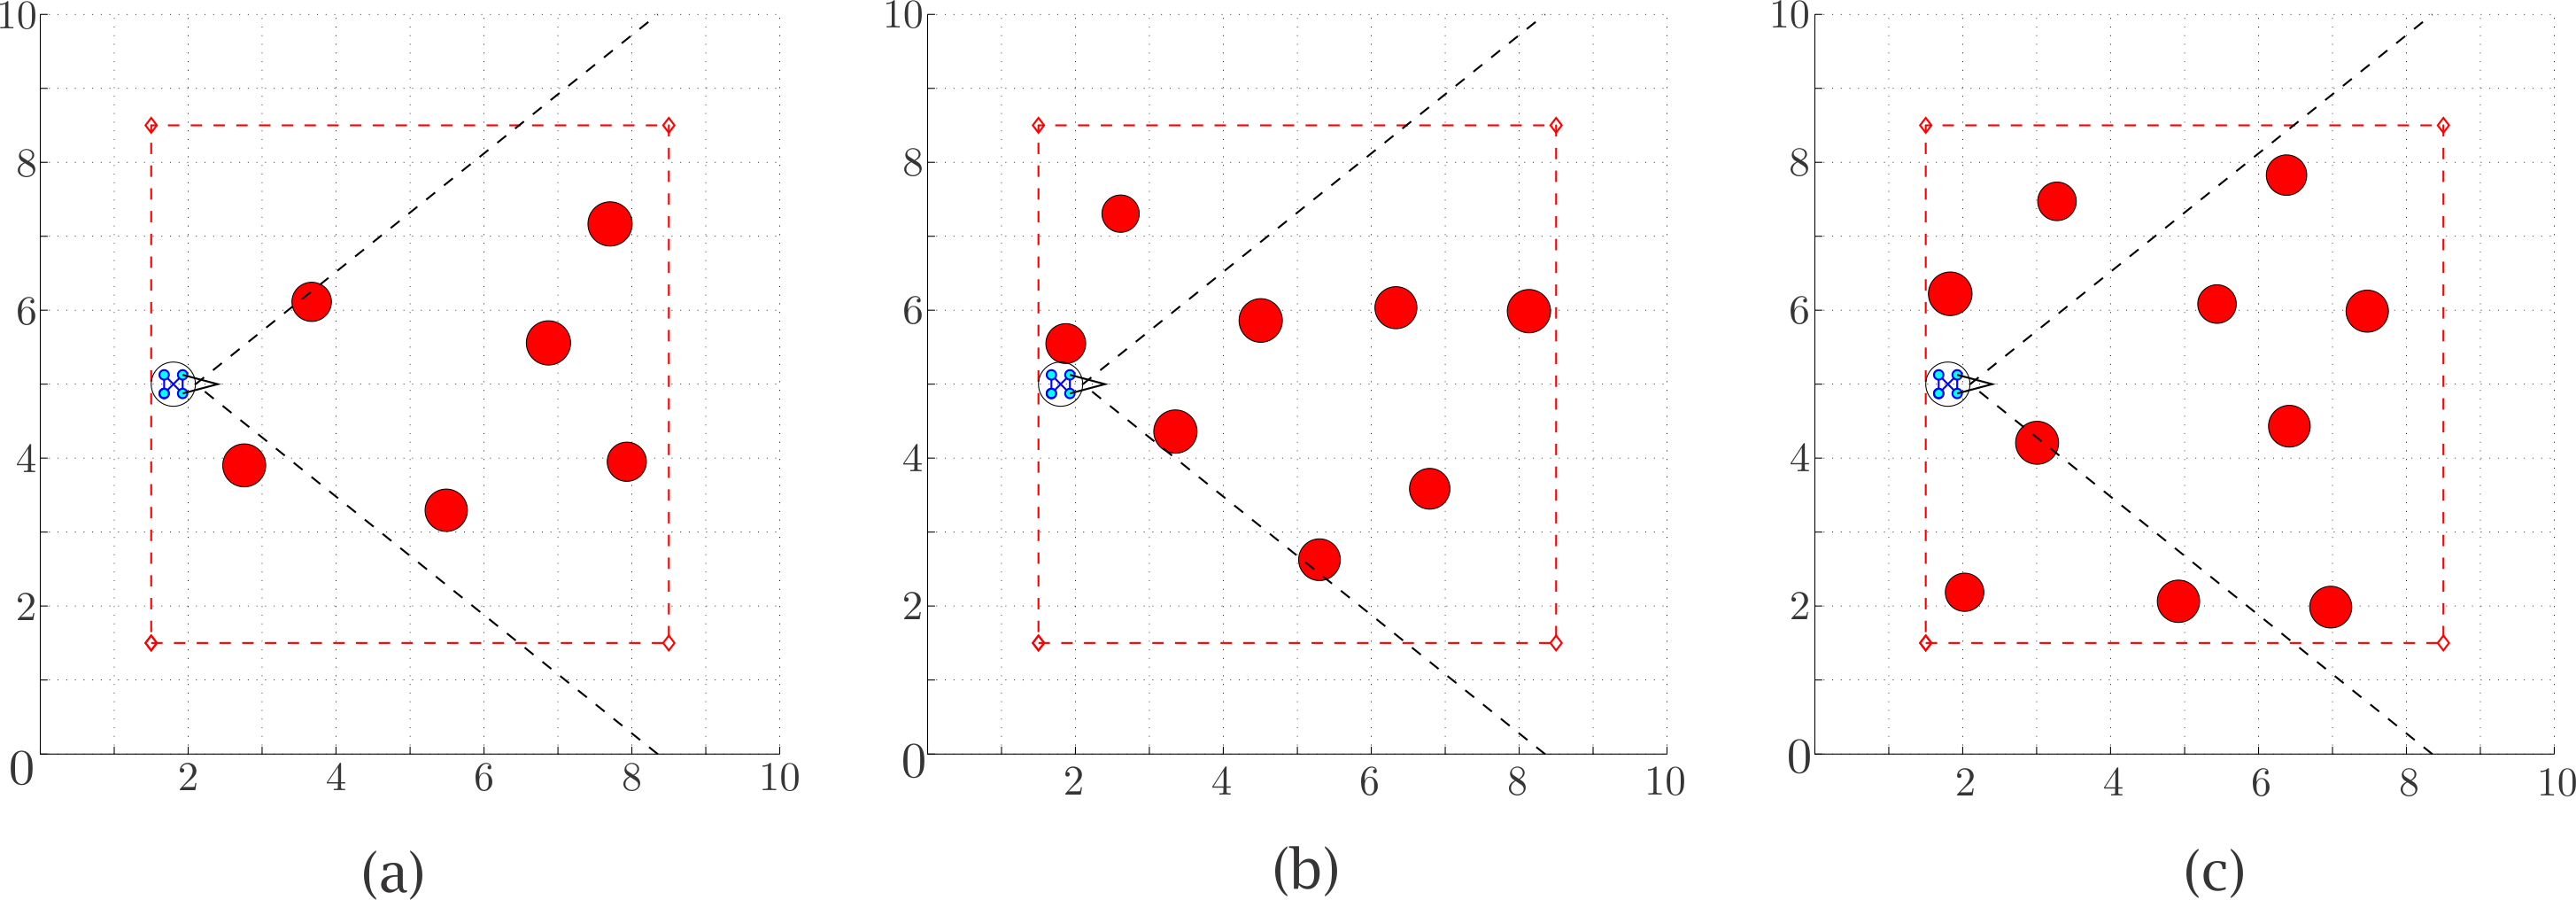
\includegraphics[width=1\linewidth]{Figures/TopViewSamples_3.png}
\centering
\caption{Three sample of obstacle random positioning in the competition field (cyberzoo), (a) with six poles, (b) with eight poles, and (c) with ten poles}
\label{f:TopViewSamples}
\end{figure} 

\begin{figure}[h]
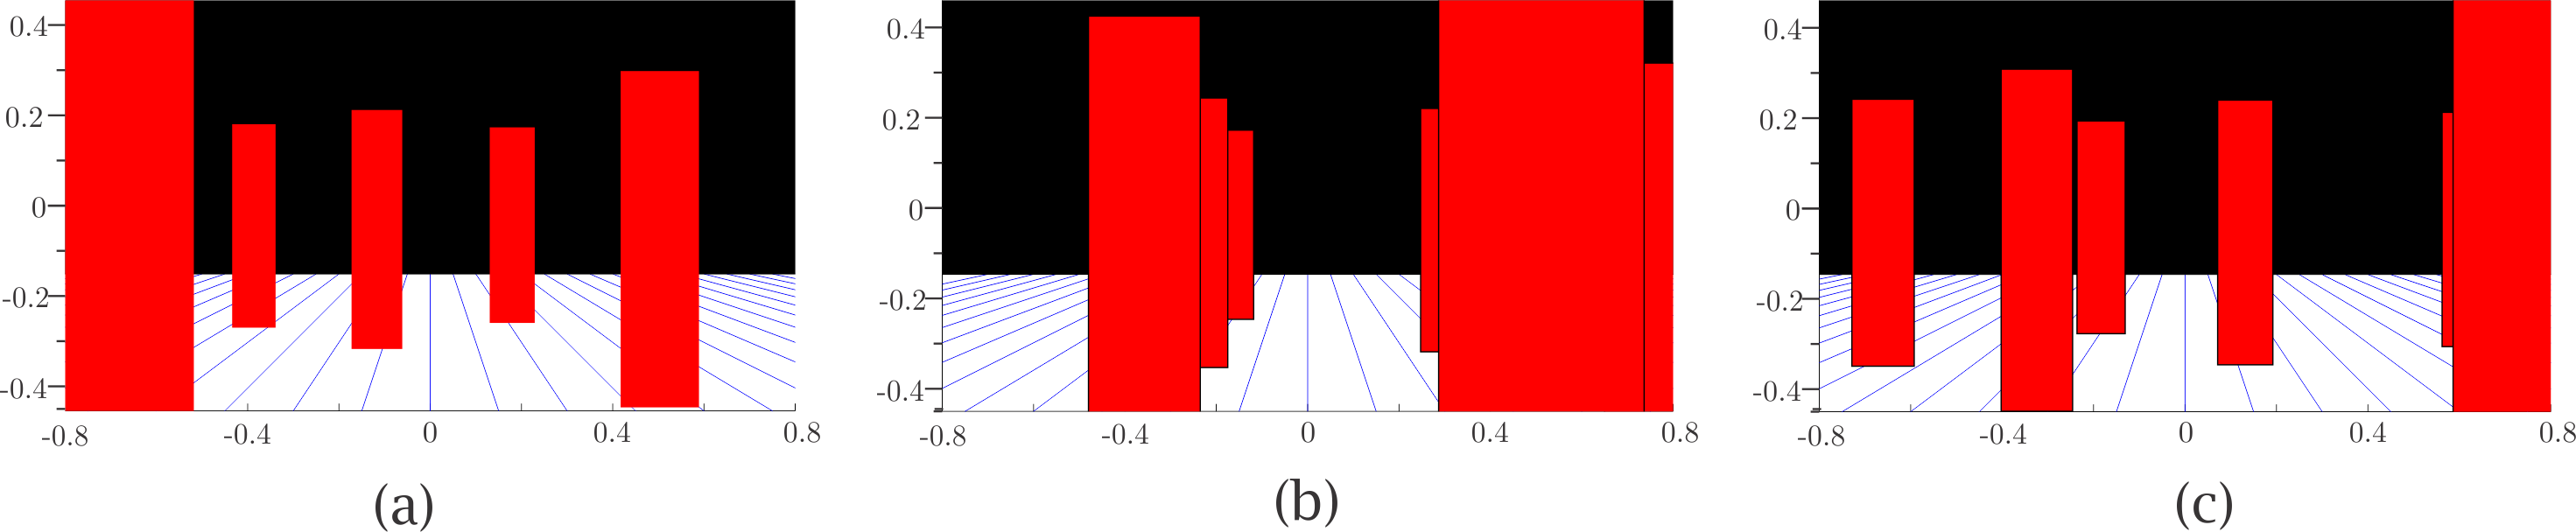
\includegraphics[width=1\linewidth]{Figures/CameraViewSamples_3.png}
\centering
\caption{Poles position as viewed by the AR.Drone front camera for (a) six poles, (b) eight poles, and (c) ten poles, corresponded to the sample (a), (b) and(c) in Figure~\ref{f:TopViewSamples}. Notice that not all poles are covered by the camera field-of-view (FOV)}
\label{f:CameraViewSamples}
\end{figure} 

\begin{figure}
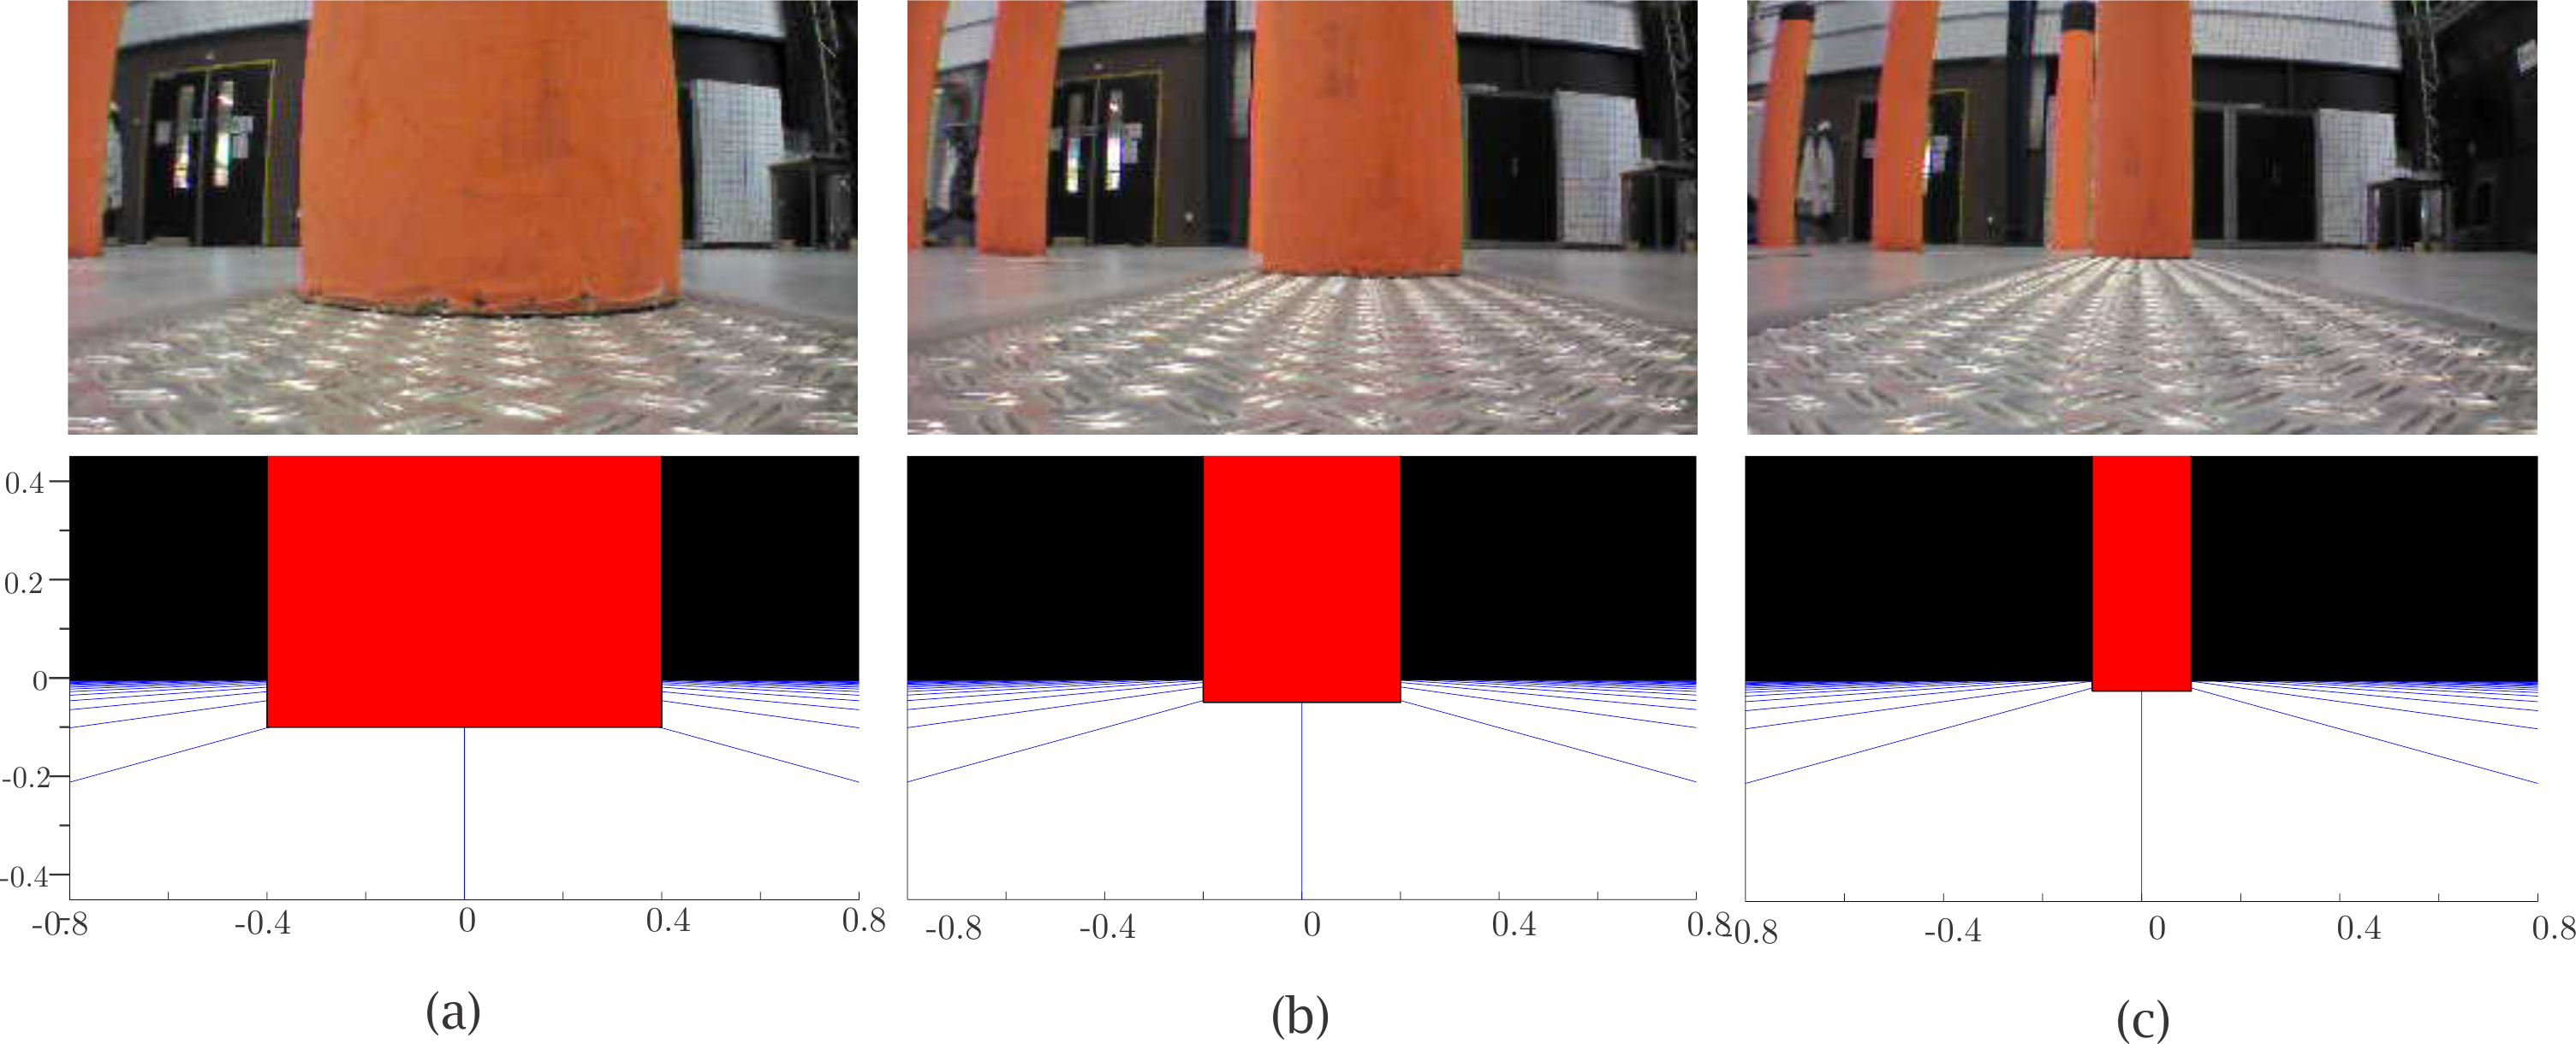
\includegraphics[width=1\linewidth]{Figures/Calibrations.png}
\centering
\caption{Calibration of the camera view model, conducted by comparing real snapshots from the AR.Drone front camera (top) with the result in the simulation (bottom). The drone on ground and a pole is positioned at (a) 0.5 meter, (b) 1 meter, and (c) two meter from the front camera.}
\label{f:Calibrations}
\end{figure} 



\subsubsection{Strategy Implementation Result}
The implemented strategy is as described in the previous section, summarized in the flow chart in Figure~\ref{fp1}. The result is shown in series of frames (time-captured) as can be observed in Figure~\ref{f:Simulation_8Poles}, for the situation where eight poles is used. The first strategy is tested in random obstacle configuration in the tournament field. The result of number of collisions, as well as covered distance, can be seen in the fourth frame. It should be noted that the result shown in this report is not the best result for the strategy proposed, since it result in four collisions. Tuning of threshold, as explained in the previous sections is required, which unfortunately have not been conducted thoroughly in this project due the limitation of time.

\begin{figure}[h]
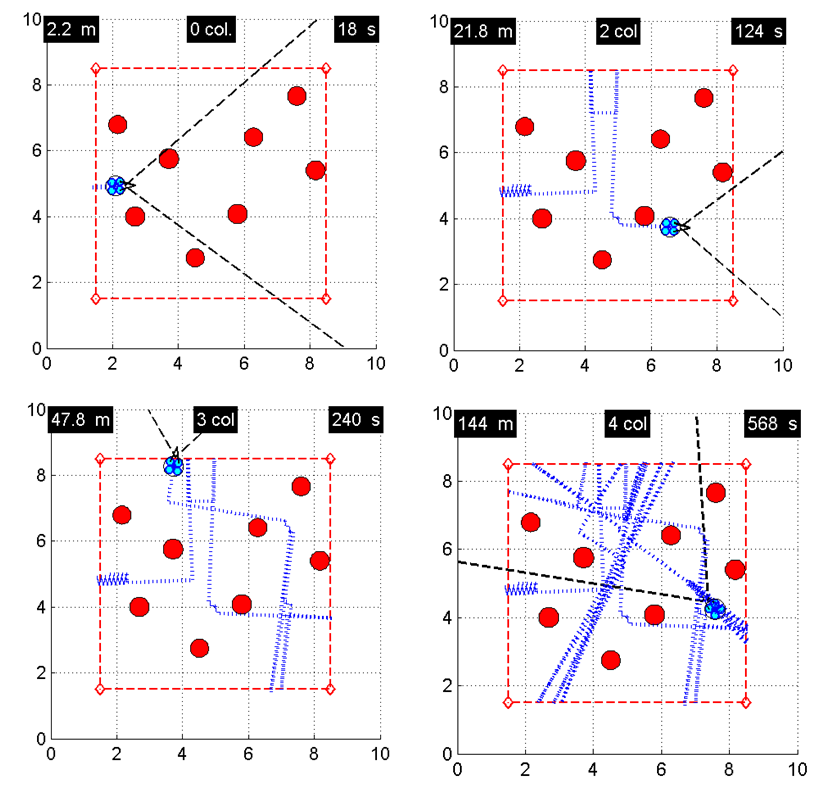
\includegraphics[width=1\linewidth]{Figures/Simulation_8Poles.png}
\centering
\caption{Simulation runs for 10 minutes, for cases with eight poles positioned in random.}
\label{f:Simulation_8Poles}
\end{figure}


